

\section{Methodology}

We propose \textit{SpiderMark}, a frequency-domain watermarking framework for diffusion-based image generation that operates entirely at the noise initialisation stage and requires no modification to pretrained model weights. 
The method consists of three tightly coupled components: (i) direct watermark injection into the initial diffusion noise, (ii) verifier dataset construction via paired watermarked and unwatermarked generations, and (iii) probabilistic watermark verification using a lightweight classifier. 
The complete pipeline is summarised and illustrated in Fig.~\ref{fig:spidernet}.


Given a pretrained diffusion model $\mathcal{G}$, SpiderMark injects a fixed, structured watermark pattern into the frequency representation of the initial latent noise prior to the denoising process. 
This design ensures full compatibility with existing diffusion models and sampling procedures while allowing the watermark signal to propagate naturally through the reverse diffusion trajectory.
To enable robust detection, we generate matched pairs of watermarked and clean images under identical prompts and noise seeds, from which frequency-domain features are extracted to train a verifier network.
At inference time, the verifier outputs a calibrated confidence score indicating the presence of the watermark in a given image.

In what follows, we first describe the watermark injection mechanism, and then detail the veri\\\fier’s training and inference procedure.


\subsection{Injection Phase}
Let \(x_T \sim \mathcal{N}(0,I)\) denote the initial Gaussian latent used to initialise the diffusion process.
SpiderMark embeds a structured watermark \(W\) directly into the frequency-domain representation of \(x_T\).
The complete injection and watermarked image generation procedure is summarised in Algorithm~\ref{alg:injection_generation}.

The Fourier transform of the latent noise is first computed as
\begin{equation}
    X_T = \mathcal{F}\{x_T\},
\end{equation}
where the transform operates over the two-dimensional spatial dimensions of the latent.
A watermark pattern is then injected into the frequency domain to balance robustness and imperceptibility:
\begin{equation}
    \tilde{X}_T = (1-\alpha)\,X_T + \alpha\,W,
\end{equation}
where \(\alpha \in [0,1]\) controls the watermark embedding strength.
The modified spectrum is subsequently transformed back to the spatial domain:
\begin{equation}
    \tilde{x}_T = \mathcal{F}^{-1}\{\tilde{X}_T\}.
\end{equation}
The resulting watermarked latent serves as the starting point for the denoising trajectory of the pretrained diffusion model, producing a final image \(\tilde{x}_0\) that implicitly carries the embedded watermark.
This strategy is lightweight and model-agnostic, requiring no modification to pretrained diffusion weights.


\begin{algorithm}[t]
\caption{Watermark Injection and Watermarked Image Generation}
\label{alg:injection_generation}
\begin{algorithmic}[1]
\Require
Pretrained diffusion model $\mathcal{G}$;
fixed frequency-domain watermark pattern $W$;
injection strength $\alpha \in [0,1]$;
prompt $\mathbf{p}$.

\Ensure
Watermarked latent noise $\tilde{x}_T$;
watermarked generated image $\tilde{x}_0$.

\State Sample initial latent noise $x_T \sim \mathcal{N}(0,I)$.
\State Compute Fourier representation $X_T \leftarrow \mathcal{F}\{x_T\}$.
\State Inject watermark in frequency domain:
\State \hspace{1.2em} $\tilde{X}_T \leftarrow (1-\alpha)X_T + \alpha W$.
\State Invert transform: $\tilde{x}_T \leftarrow \mathcal{F}^{-1}\{\tilde{X}_T\}$.
\State Generate watermarked image: $\tilde{x}_0 \leftarrow \mathcal{G}(\tilde{x}_T, \mathbf{p})$.
\end{algorithmic}
\end{algorithm}


\paragraph{Spider-web Pattern Generation.}
The watermark \(W(u,v)\) is generated as a regular spider-web pattern that consists of \(n_s\) evenly spaced radial spokes and \(n_\ell\) polygonal ring connectors.  
Let the image dimensions be \(H \times W\), and let the center coordinates be \((x_c,y_c)=(W/2,H/2)\).  
For each spoke \(i \in \{1,\ldots,n_s\}\), we define the angle
\begin{equation}
    \theta_i = \frac{2\pi(i-1)}{n_s},
\end{equation}
and for each ring level \(k \in \{1,\ldots,n_\ell\}\) we define a normalized radius
\begin{equation}
    r_k = r_{\max}\!\left(\frac{k}{n_\ell}\right), \quad r_{\max} = \tfrac{1}{2}\min(H,W)\,\rho,
\end{equation}
where \(\rho\in(0,1)\) determines the overall size of the web relative to the canvas.  
The coordinates of each web node are
\begin{equation}
    (x_{i,k},y_{i,k}) = (x_c + r_k\cos\theta_i,\; y_c + r_k\sin\theta_i).
\end{equation}
Each spoke is represented as a line segment from \((x_c,y_c)\) to \((x_{i,n_\ell},y_{i,n_\ell})\),  
and each ring is formed by connecting adjacent spokes:
\begin{equation}
    (x_{i,k},y_{i,k}) \longleftrightarrow (x_{i+1,k},y_{i+1,k}),
\end{equation}
with \(x_{n_s+1,k}=x_{1,k}\) to close the loop.  
The resulting binary mask \(M(x,y)\in\{0,1\}\) is normalized as
\begin{equation}
    W(u,v)=\frac{M(x,y)-\mu_M}{\sigma_M},
\end{equation}
to form a zero-mean, unit-variance carrier before frequency-space blending.

\paragraph{Advantages of the Spider-web Pattern.}
Most existing watermarking techniques employ simple geometric or frequency-based designs such as concentric rings, grids, or random masks. These isotropic structures distribute watermark energy uniformly by radius, making them vulnerable to directional distortions such as motion blur, anisotropic resampling, or compression artifacts.  

The spider-web pattern introduces both radial and angular components, forming an interconnected lattice of concentric rings and vertical spokes. This structure offers several key advantages:
\begin{itemize}
    \item \textit{Directional robustness:} Energy distributed across vertical, horizontal, and diagonal orientations resists directionally biased degradations, unlike circular-only ring patterns.
    \item \textit{Spatial redundancy:} The spokes connect low- and mid-frequency regions, preserving partial watermark cues even under cropping or localized corruption.
    \item \textit{Frequency balance:} Vertical and diagonal components overlap slightly with low-frequency bands near the spectral center, providing improved robustness without introducing visible global distortion.
\end{itemize}
Together, these properties make the spider-web watermark more resilient, interpretable, and visually imperceptible than conventional ring-based approaches, enhancing content attribution in diffusion-generated imagery.

\subsection{Verification Phase.}

The verification phase determines whether a given image contains a watermark. Traditional verification methods typically rely on handcrafted similarity or distance metrics, such as correlation or spectral energy comparisons. While effective on clean images, these approaches degrade substantially under common attacks, including cropping and geometric distortions. SpiderMark instead adopts a learned verifier operating in the frequency domain, designed to detect the subtle and structured spectral signatures induced by the injected watermark. In addition, auxiliary similarity cues, including L1 distance and PSNR, are provided to the verifier to further enhance detection robustness. This learned formulation generalises well to unseen perturbations and maintains strong detection performance under real-world image transformations.


\paragraph{Verifier Training Dataset ($\mathcal{D}$) Construction.}


\begin{algorithm}[t]
\caption{{\color{blue}Verifier Training Dataset Construction}}
\label{alg:verifier_dataset}
\begin{algorithmic}[1]
\Require
Pretrained diffusion model $\mathcal{G}$;
frequency-domain watermark pattern $W$;
injection strength $\alpha$;
prompt set $\mathcal{P}$;
number of prompts $N$.

\Ensure
Verifier training set $\mathcal{D}$ of labeled images.

\State Initialize dataset $\mathcal{D} \leftarrow \emptyset$.
\For{$i = 1$ to $N$}
    \State Sample prompt $\mathbf{p}_i \sim \mathcal{P}$ and latent noise $x_T^{(i)} \sim \mathcal{N}(0,I)$.
    \State Generate clean image: $x_0^{(i)} \leftarrow \mathcal{G}(x_T^{(i)}, \mathbf{p}_i)$.

    \State Compute spectrum: $X_T^{(i)} \leftarrow \mathcal{F}\{x_T^{(i)}\}$.
    \State Inject watermark in frequency domain:
    \State \hspace{1.2em} $\tilde{X}_T^{(i)} \leftarrow (1-\alpha)X_T^{(i)} + \alpha W$.
    \State Invert transform: $\tilde{x}_T^{(i)} \leftarrow \mathcal{F}^{-1}\{\tilde{X}_T^{(i)}\}$.
    \State Generate watermarked image: $\tilde{x}_0^{(i)} \leftarrow \mathcal{G}(\tilde{x}_T^{(i)}, \mathbf{p}_i)$.

    \State Add labeled image samples:
    \State \hspace{1.2em} $\mathcal{D} \leftarrow \mathcal{D} \cup \{(x_0^{(i)},0), (\tilde{x}_0^{(i)},1)\}$.
\EndFor
\end{algorithmic}
\end{algorithm}

To train the watermark verifier, we construct a paired dataset of clean and watermarked images generated under identical prompts and latent noise initialisations. 
This controlled pairing ensures that the verifier learns to detect watermark-induced spectral signatures, rather than spurious differences arising from semantic content or prompt variation.

Specifically, for each sampled prompt, we draw a single latent noise realisation and use it to generate two images: a clean image produced from the original noise, and a watermarked image generated from the corresponding noise after frequency-domain watermark injection. 
Both images are produced using the same pretrained diffusion model, guaranteeing consistency across all other factors.

The resulting dataset consists of labeled image pairs, where clean images are assigned label~$0$ and watermarked images are assigned label~$1$. Algorithm~\ref{alg:verifier_dataset} summarises the verifier dataset construction procedure.


\paragraph{Verifier Training.}
The verification network $f_{\theta}$ is trained as a binary classifier to distinguish between watermarked and non-watermarked images.
An overview of the training phase is shown in the bottom part of Fig.~\ref{fig:spidernet}, and the verifier architecture is illustrated in Fig.~\ref{fig:veifier_arch}.
The complete training procedure is summarised in Algorithm~\ref{alg:verifier_training}.

The network is optimised using the binary cross-entropy loss
\begin{equation}
    \mathcal{L} = - \frac{1}{N} \sum_{i=1}^{N}
    \left[y_i \log f_{\theta}(x_i) + (1 - y_i)\log(1 - f_{\theta}(x_i))\right],
\end{equation}
where $y_i \in \{0,1\}$ indicates the presence of a watermark.
The verifier outputs a confidence score $p_i = f_{\theta}(x_i)$, which is thresholded at $0.5$ to obtain a binary prediction.

By combining learned spectral representations with explicit similarity cues based on $\ell_1$ distance and PSNR, SpiderMark leverages both data-driven feature learning and handcrafted watermark-aligned measures.


\begin{algorithm}[t]
\caption{{\color{blue}Verifier Training}}
\label{alg:verifier_training}
\begin{algorithmic}[1]
\Require
Verifier network $f_\theta$;
loss function $\ell$ (binary cross-entropy);
optimiser \textsc{Opt};
epochs $E$;
batch size $B$;
training set $\mathcal{D} = \{(x^{(i)}, y^{(i)})\}_{i=1}^{2N}$,
where $x^{(i)} \in \{x_0^{(k)}, \tilde{x}_0^{(k)}\}$ and $y^{(i)} \in \{0,1\}$.

\Ensure
Trained verifier parameters $\theta$.

\For{$e = 1$ to $E$}
    \For{each mini-batch $\mathcal{B} = \{(x^{(j)}, y^{(j)})\}_{j=1}^{B}$ sampled from $\mathcal{D}$}
        \State Compute predictions: $\hat{y}^{(j)} \leftarrow f_\theta(x^{(j)})$ for all $(x^{(j)},y^{(j)}) \in \mathcal{B}$.
        \State Compute loss: $\mathcal{L} \leftarrow \frac{1}{B}\sum_{j=1}^{B}\ell(\hat{y}^{(j)}, y^{(j)})$.
        \State Update parameters: $\theta \leftarrow \textsc{Opt}(\theta, \nabla_\theta \mathcal{L})$.
    \EndFor
\EndFor
\end{algorithmic}
\end{algorithm}

\begin{figure*}
    \centering
    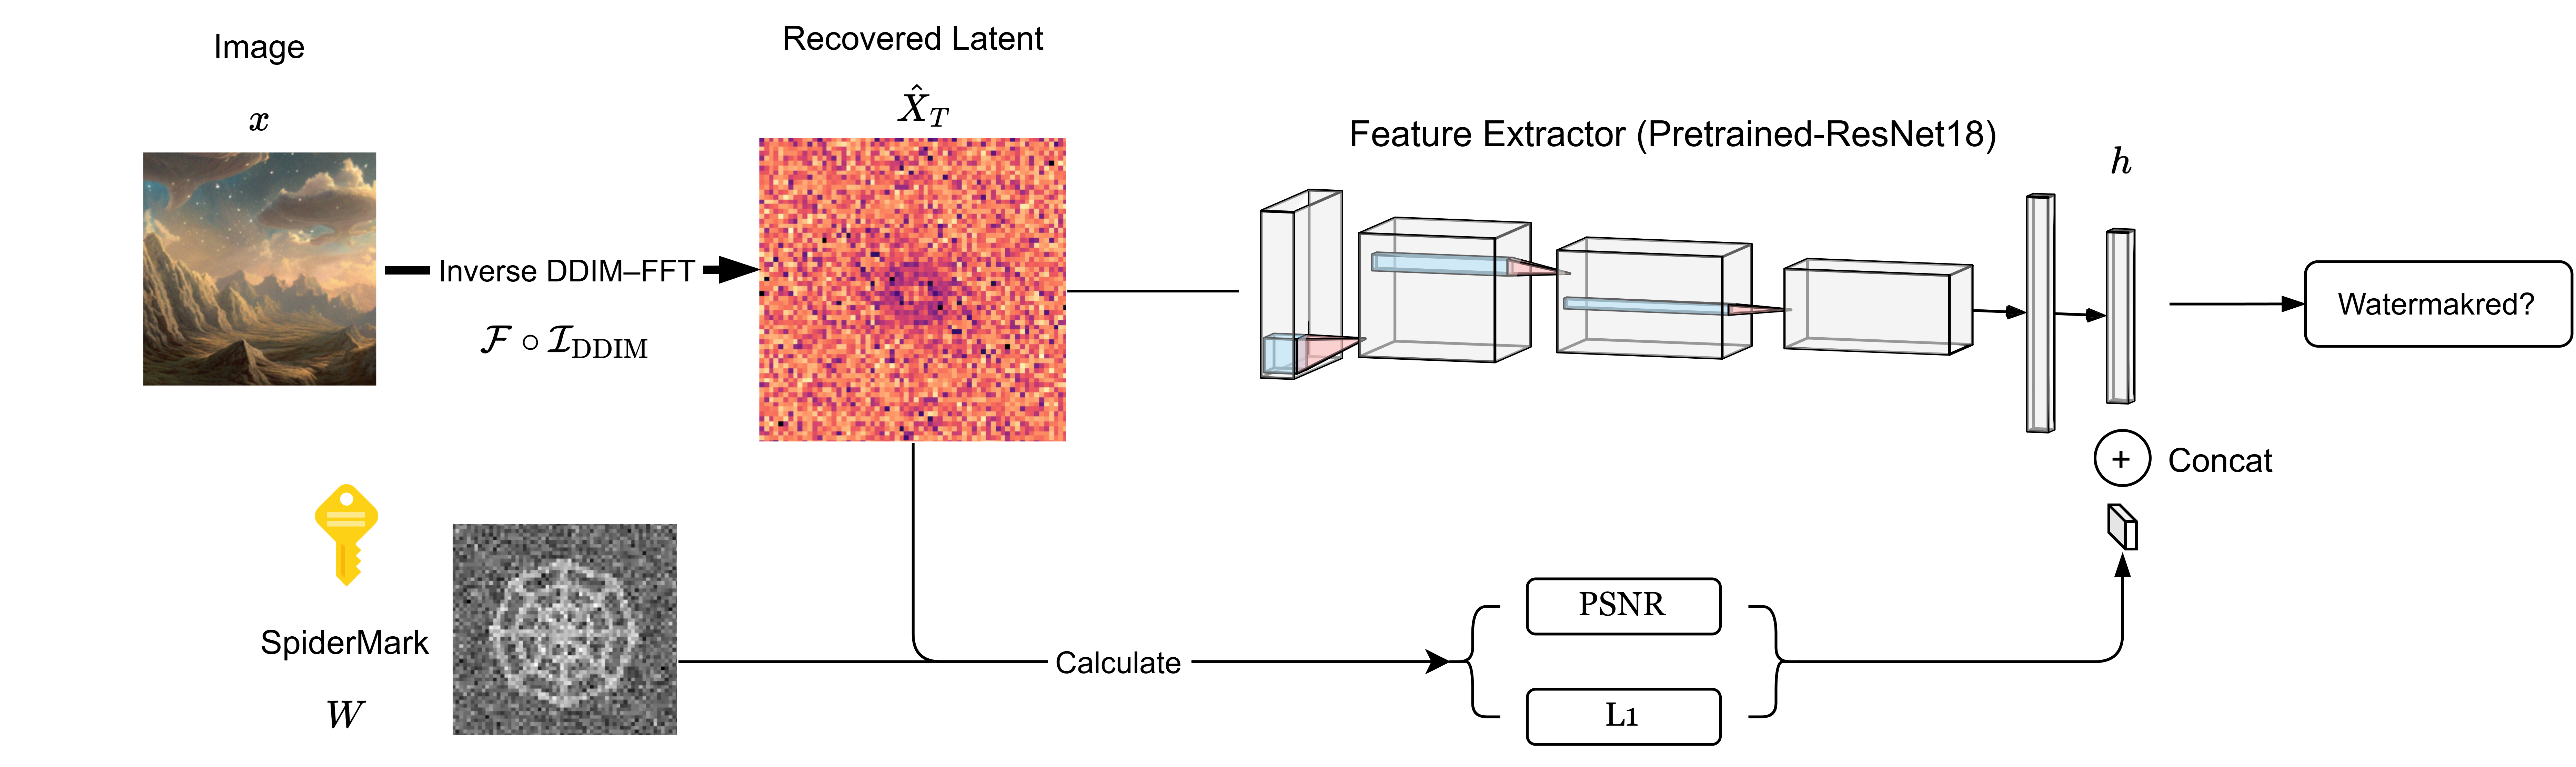
\includegraphics[width=1\linewidth]{figures/verifier_arch.png}
    \caption{{\color{blue}Verifier ($f_\theta$) Architecture. Given an input image, we first recover its corresponding watermark latent via inverse DDIM followed by a Fourier transform. The resulting frequency-domain representation is processed by a pretrained ResNet-18 verifier, augmented with auxiliary similarity cues (PSNR and L1) computed against the fixed SpiderMark pattern. The verifier outputs a probabilistic prediction indicating whether the image is watermarked.}}
    \label{fig:veifier_arch}
\end{figure*}


% \paragraph{Watermark Verification (Inference).}

% Given a query image $x$, SpiderMark determines the presence of the embedded watermark through a lightweight inference procedure that operates entirely in the frequency domain.
% Unlike injection and dataset construction, the verification stage does not require access to prompts, noise seeds, or the diffusion generator.

% For verification, we apply the inverse DDIM procedure corresponding to the same pretrained diffusion model used during generation.
% We treat inverse DDIM as a deterministic operator that approximately recovers the terminal latent noise from a generated image.
% Let $\mathcal{I}_{\text{DDIM}}(\cdot)$ denote this inverse mapping, and compute
% \begin{equation}
%     \hat{x}_T = \mathcal{I}_{\text{DDIM}}(x).
% \end{equation}

% The recovered latent $\hat{x}_T$ is transformed into the frequency domain via a two-dimensional Fourier transform,
% \begin{equation}
%     \hat{X}_T = \mathcal{F}\{\hat{x}_T\},
% \end{equation}
% where $(u,v)$ index the vertical and horizontal spatial-frequency components.
% We construct the verifier input as the magnitude spectrum
% \begin{equation}
%     S(u,v) = \left|\hat{F}_T(u,v)\right|,
% \end{equation}
% which captures the spectral footprint induced by watermark injection while discarding phase information that is less stable under image perturbations.

% Since SpiderMark embeds a fixed and known watermark pattern $W(u,v)$ during injection, we additionally compute explicit similarity measures between the recovered spectrum and the reference pattern.
% Specifically, we compute a masked $\ell_1$ distance
% \begin{equation}
%     d_{\ell_1} = \frac{1}{\|M\|_1} \left\| M \odot \left(S - W\right) \right\|_1,
% \end{equation}
% and a masked peak signal-to-noise ratio (PSNR),
% \begin{equation}
%     \mathrm{PSNR}_M = 10 \log_{10} \left( \frac{\mathrm{MAX}^2}{\mathrm{MSE}_M + \epsilon} \right),
% \end{equation}
% where
% \begin{equation}
%     \mathrm{MSE}_M = \frac{1}{\|M\|_1} \left\| M \odot \left(S - W\right) \right\|_2^2.
% \end{equation}
% Here, $M(u,v)$ denotes a binary mask defining the watermark support in the frequency domain, $\mathrm{MAX}$ is the maximum possible value of the normalized spectrum magnitude, and $\epsilon$ is a small constant for numerical stability.

% Finally, the magnitude spectrum $S(u,v)$ is processed by a convolutional backbone $\phi(\cdot)$ to extract deep frequency-domain features.
% The resulting feature embedding is concatenated with the two scalar similarity cues $(\mathrm{PSNR}_M, d_{\ell_1})$ and passed to a lightweight verifier head, which outputs a calibrated watermark confidence score $p \in [0,1]$.
% A binary verification decision is obtained by thresholding $p$ at a fixed operating point $\tau$.
% The complete inference procedure is summarised in Algorithm~\ref{alg:verification_inference}.


% \begin{algorithm}[t]
% \caption{Watermark Verification (Inference)}
% \label{alg:verification_inference}
% \begin{algorithmic}[1]
% \Require
% Query image $x$;
% inverse DDIM operator $\mathcal{I}_{\text{DDIM}}(\cdot)$;
% Fourier transform $\mathcal{F}(\cdot)$;
% reference watermark pattern $W$ and mask $M$;
% feature extractor $\phi(\cdot)$;
% trained verifier $f_\theta(\cdot)$;
% decision threshold $\tau$.

% \Ensure
% Watermark confidence $p \in [0,1]$;
% verification decision $\mathbb{1}[p \ge \tau]$.

% \State Recover terminal latent noise: $\hat{x}_T \leftarrow \mathcal{I}_{\text{DDIM}}(x)$.
% \State Compute spectrum magnitude: $S \leftarrow \left| \mathcal{F}\{\hat{x}_T\} \right|$.

% \State Compute masked $\ell_1$ similarity:
% \State \hspace{1.2em} $d_{\ell_1} \leftarrow \frac{1}{\|M\|_1} \left\| M \odot (S - W) \right\|_1$.
% \State Compute masked PSNR:
% \State \hspace{1.2em} $\mathrm{MSE}_M \leftarrow \frac{1}{\|M\|_1} \left\| M \odot (S - W) \right\|_2^2$.
% \State \hspace{1.2em} $\mathrm{PSNR}_M \leftarrow 10 \log_{10}\!\left(\frac{\mathrm{MAX}^2}{\mathrm{MSE}_M + \epsilon}\right)$.

% \State Extract deep features: $h \leftarrow \phi(S)$.
% \State Fuse cues and predict: $p \leftarrow f_\theta\!\left([h;\ \mathrm{PSNR}_M;\ d_{\ell_1}]\right)$.
% \State Output decision: $\mathbb{1}[p \ge \tau]$.
% \end{algorithmic}
% \end{algorithm}



{\color{blue}
\paragraph{Watermark Verification (Inference).}

Given a query image $x$, SpiderMark determines the presence of the embedded watermark through a lightweight inference procedure that operates in the frequency domain.
Unlike injection and dataset construction, the verification stage does not require access to prompts, noise seeds, or the diffusion generator.

For verification, we apply the inverse DDIM procedure corresponding to the same pretrained diffusion model and noise schedule used during generation.
We treat inverse DDIM as a deterministic operator that approximately recovers the terminal latent noise from a generated image.
Let $\mathcal{I}_{\text{DDIM}}(\cdot)$ denote this inverse mapping, and compute
\begin{equation}
    \hat{x}_T = \mathcal{I}_{\text{DDIM}}(x).
\end{equation}

The recovered latent $\hat{x}_T$ is transformed into the frequency domain via a two-dimensional Fourier transform,
\begin{equation}
    \hat{X}_T = \mathcal{F}\{\hat{x}_T\},
\end{equation}

Since SpiderMark embeds a fixed and known watermark pattern $W$ during injection, we additionally compute explicit similarity measures between the recovered spectrum and the reference pattern within the watermark support.
Let $M(u,v)$ denote a binary mask defining the watermark support in the frequency domain.
We compute a masked $\ell_1$ distance
\begin{equation}
    d_{\ell_1} = \frac{1}{\|M\|_1}\left\| M \odot \left(\hat{X}_T - W\right) \right\|_1,
\end{equation}
and a masked peak signal-to-noise ratio (PSNR),
\begin{equation}
    \mathrm{PSNR}_M = 10 \log_{10}\!\left( \frac{\mathrm{MAX}^2}{\mathrm{MSE}_M + \epsilon} \right),
\end{equation}
where
\begin{equation}
    \mathrm{MSE}_M = \frac{1}{\|M\|_1}\left\| M \odot \left(\hat{X}_T - W\right) \right\|_2^2.
\end{equation}
Here, $\mathrm{MAX}$ denotes the maximum possible value of the normalized real-valued representation of $\hat{X}_T$, and $\epsilon$ is a small constant for numerical stability.

Finally, the recovered spectrum $\hat{X}_T$ is processed by the verifier network $f_\theta(\cdot)$, which internally extracts deep frequency-features and fuses them with the two scalar similarity cues $(\mathrm{PSNR}_M, d_{\ell_1})$ in its final prediction layer.
Concretely, the backbone of $f_\theta$ produces an embedding $h$, which is concatenated with $(\mathrm{PSNR}_M, d_{\ell_1})$ and fed into the last layer to output a calibrated watermark confidence score $p \in [0,1]$.
A binary verification decision is obtained by thresholding $p$ at a fixed operating point $\tau$.
The complete inference procedure is summarised in Algorithm~\ref{alg:verification_inference}.

\begin{algorithm}[t]
\caption{Watermark Verification (Inference)}
\label{alg:verification_inference}
\begin{algorithmic}[1]
\Require
Query image $x$;
inverse DDIM operator $\mathcal{I}_{\text{DDIM}}(\cdot)$;
Fourier transform $\mathcal{F}\{\cdot\}$;
reference watermark pattern $W$ and mask $M$;
trained verifier $f_\theta(\cdot)$;
normalization constant $\mathrm{MAX}$;
stability constant $\epsilon$;
decision threshold $\tau$.

\Ensure
Watermark confidence $p \in [0,1]$;
verification decision $\mathbb{1}[p \ge \tau]$.

\State Recover terminal latent noise: $\hat{x}_T \leftarrow \mathcal{I}_{\text{DDIM}}(x)$.
\State Compute Fourier spectrum: $\hat{X}_T \leftarrow \mathcal{F}\{\hat{x}_T\}$.

\State Compute masked $\ell_1$ similarity:
\State \hspace{1.2em} $d_{\ell_1} \leftarrow \frac{1}{\|M\|_1}\left\| M \odot (\hat{X}_T - W) \right\|_1$.
\State Compute masked PSNR:
\State \hspace{1.2em} $\mathrm{MSE}_M \leftarrow \frac{1}{\|M\|_1}\left\| M \odot (\hat{X}_T - W) \right\|_2^2$.
\State \hspace{1.2em} $\mathrm{PSNR}_M \leftarrow 10 \log_{10}\!\left(\frac{\mathrm{MAX}^2}{\mathrm{MSE}_M + \epsilon}\right)$.

\State Predict watermark confidence (fusion occurs in the last layer of $f_\theta$):
\State \hspace{1.2em} $p \leftarrow f_\theta(\hat{X}_T, \mathrm{PSNR}_M, d_{\ell_1})$.
\State Output decision: $\mathbb{1}[p \ge \tau]$.
\end{algorithmic}
\end{algorithm}
}